\documentclass[9pt,twoside,lineno]{pnas-new}
% Use the lineno option to display guide line numbers if required.

\templatetype{pnassupportinginfo}

% Math
\def\P{\mathbb{P}}
\def\cor{\mathrm{cor}}
\def\Quantile{\mathrm{Quantile}}
\def\logit{\mathrm{logit}}
\def\dist{\mathrm{dist}}
\def\WIS{\mathrm{WIS}}
\def\AUC{\mathrm{AUC}}
\def\CCF{\mathrm{CCF}}
\newcommand{\indicator}[1]{\mathbf{1}\left(#1\right)}

% Figures and tables
\usepackage{xurl}
\usepackage{microtype}
\usepackage{booktabs}
\usepackage{caption}
\usepackage{subcaption}
\usepackage{xcolor}
\newcommand{\attn}[1]{\textcolor{red}{[ATTN: #1]}}

\makeatletter 
\renewcommand\@biblabel[1]{#1} 
\makeatother

% indicators
\newcommand{\chngcli}{CHNG-CLI}
\newcommand{\chngcov}{CHNG-COVID}
\newcommand{\dv}{DV-CLI}
\newcommand{\ar}{AR}
\newcommand{\fb}{CTIS-CLI-in-community}
\newcommand{\gs}{Google-AA}


\providecommand{\tightlist}{%
  \setlength{\itemsep}{0pt}\setlength{\parskip}{0pt}}


\title{Can Auxiliary Indicators Improve COVID-19 Forecasting and Hotspot  
  Prediction?} 

\author{Daniel J. McDonald, Jacob Bien, Alden Green, Addison J. Hu, Nat DeFries,
  Sangwon Hyun, Natalia L. Oliveira, James Sharpnack, Jingjing Tang, Robert
  Tibshirani, Valerie Ventura, Larry Wasserman, and Ryan J. Tibshirani} 
\correspondingauthor{Daniel J. McDonald.\\E-mail: daniel@stat.ubc.ca}

\begin{document}

\maketitle


\SItext



\section{Finalized Versus Vintage Data}

The goal of this section is to quantify the effect of not properly accounting
for the question of ``what was known when'' in performing retrospective
evaluations of forecasters.  Figures \ref{fig:fcast-finalized} and
\ref{fig:hot-finalized} show what Figures 3 and 4 in the main paper would have
looked like if we had simply trained all models using the finalized data rather
than using vintage data.  This comparison can be seen more straightforwardly in
Figures \ref{fig:fcast-honest-v-finalized} and \ref{fig:hot-honest-v-finalized},
which show the ratio in performance between the vintage and finalized versions.
When methods are given the finalized version of the data rather than the version
available at the time that the forecast would have been made, all methods appear
(misleadingly) to have better performance than they would have had if run
prospectively.  For example, for forecasting case rates 7-days ahead, the WIS of
all methods is at least 8\% larger than what would have been achieved using
finalized data.  This effect diminishes as the forecasting horizon increases,
reflecting the fact that longer-horizon forecasters rely less heavily on recent
data than very short-horizon forecasters.  Crucially, some methods are
``helped'' more than others by the less scrupulous retrospective evaluation,
underscoring the difficulty of avoiding misleading conclusions when performing
retrospective evaluations of forecasters.

\chngcli~(and, to a lesser extent, the other claims-based signals) is the most
affected by this distinction, reflecting the latency in claims-based reporting.
This underscores the importance of efforts to provide ``nowcasts'' for claims
signals (which corresponds to a 0-ahead forecast of what the claims signal's
value will be once all data has been collected). Looking at the \chngcli~and
\dv~curves in Figure \ref{fig:fcast-finalized}, we can see that they perform
very similarly when trained on the finalized data.  This is reassuring because
they are, in principle, measuring the same thing (namely, the percentage of
outpatient visits that are primarily about COVID-related symptoms), but based on
data from different providers.  The substantial difference in their curves in
Figure 3 of the main paper must therefore reflect their having very different
backfill profiles. 
  
While using finalized rather than vintage data affects \dv~the least for
forecasting, it is one of the most affected methods for the hotspot problem.
This is a reminder that the forecasting and hotspot problems are fundamentally
different problems.  For example, the hotspot problem does not measure the
ability to distinguish between flat and downward trends.

Even the \ar~model is affected by this distinction, reflecting the fact that the
case rates themselves (i.e., the response values) are also subject to revision.
The forecasters based on indicators are thus affected both by revisions to the
indicators and by revisions to the case rates.  And in the case of the
\gs~model, in which we only used finalized values for the \gs~indicator, the
difference in performance can be wholly attributed to revisions of case rates. 

\section{Robust Aggregation}

In this section, we consider using the geometric mean instead of the usual
(arithmetic) mean when aggregating the weighted interval score (WIS) across
location-time pairs.  Aside from the geometric mean being generally more robust
to large values, there are two reasons why using it may be desirable.  

\begin{enumerate}
\item WIS is right-skewed, being bounded below by zero and having occasional 
  very large values.  Figure \ref{fig:wis-densities} illustrates that the
  densities appear roughly log-Gaussian.  The geometric mean is a natural choice   
  in such a context since it can be viewed as a measure of centrality on the log
  scale (it is the exponential of the arithmetic mean of log values).
\item In the main paper, we report the ratio of the mean WIS of a forecaster to
  the mean WIS of the baseline forecaster. Another choice could be to take the
  mean of the ratio of WIS values for the two methods. This latter choice would
  penalize a method less for doing poorly where the baseline forecaster also
  does poorly.\footnote{In a sense, this is implicitly estimating a
    nonparametric space-time effect for forecaster error, and assuming that has
    a shared, multiplicative contribution to forecaster errors.  That is, if one
    imagines that a forecaster's WIS is composed of multiplicative space-time
    effects $S_{\ell,t}$ shared across all forecasters,
    \smash{$\WIS(F_{\ell,t,f},Y_{\ell,t}) = S_{\ell,t} E_{f,t}$} with
    \smash{$E_{f,t}$} a forecaster-specific error, then taking the ratio of
    individual WIS values cancels these space-time effects.}  Using instead the
  geometric mean makes the order of aggregation and scaling immaterial since the
  ratio of geometric means is the same as the geometric mean of ratios.
\end{enumerate}

Figure \ref{fig:fcast-adjusted} uses the geometric mean for aggregation.
Comparing this with Figure 3 in the main paper, we see that the main conclusions
are largely unchanged; however, \chngcli~now appears better than \ar.  This
behavior would be expected if \chngcli's poor performance is attributable to a
relatively small number of large errors (as opposed to a large number of
moderate errors).  Indeed, Figure 5 of the main paper further corroborates this,
in which we see the heaviest left tails occur for \chngcli.

\section{Comparing COVID-19 Forecast Hub Models}

Since July of 2020, modelers have been submitting real-time forecasts of
COVID-19 case incidence to the COVID-19 Forecast Hub \cite{ForecastHub}. This 
(along with forecasts of hospitalizations and deaths collected in the same Hub)
serves as the source of the CDC's official communications on COVID forecasting. 

Our goal in this section is to compare the AR model and indicator models to
those in the Hub, in terms of forecast errors aggregated over the same forecast
tasks, to give a clear sense for how robust and effective the models we choose
to investigate in the paper are relative to those in common operational use.
This was prompted by a question from an anonymous reviewer of this paper, who
asked why we chose to build our analysis of indicator utility around the AR
model in the first place, and why we did not build it around others (say, the
SIR model or more complex mechanistic models of disease transmission) that have 
occupied more of the spotlight over the course of the pandemic.  The analysis
presented here corroborates the claim that, while simple, the AR model, properly
trained---using a quantile loss to directly estimate multiple conditional
quantiles, a trailing training window of 21 days, pooling across all locations
jointly, and fitting to case rates rather than counts (as we do in all our
models in the main paper)---can be robust and effective, performing
competitively many of the top models from COVID-19 Forecast Hub, including the
Hub ensemble model.

The closest forecast target in the Hub to that used in the main paper is 
state-level case incidence over an epiweek---defined by the sum of new case
counts reported between a Sunday and the following Saturday (inclusive). Our
forecast target, recall, is a 7-day trailing average of COVID-19 case incidence
rates at the HRR level, which is different in three regards:

\begin{enumerate}
\item temporal resolution (daily versus weekly);
\item geographic resolution (HRRs versus states); 
\item scale (rates versus counts).
\end{enumerate}

While the first and third of these differences could be easily addressed post 
hoc---meaning, we can take always take our model's output and multiply it by 
7 in order to track the incidence over any given trailing week, and rescale it
per location by population to bring it to the count scale---the second
difference is not easy to adjust post hoc due to nonlinearity of the quantiles
(a quantile of a linear combination of random variables is not simply the linear
combination of their quantiles, but rather, depends intricately on the
correlations between the random variables).    

Therefore, to make a comparison to models in the Hub as direct as possible, we
retrained our models over the same forecast period as in the main paper, and
with the same general setup entirely, except at the state rather than HRR level.
We then rescaled them post hoc to account for the different temporal resolution
and the rate versus count scale (first and third points in the above list).  The
results are given in Figure \ref{fig:compare-to-hub}.  The evaluation was
carried out exactly as in the main paper, and the figure displays both mean WIS
and geometric mean WIS, as a function of ahead, relative to the baseline model.
Furthermore, to account for missingness (not all teams submitted forecasts to
the Hub for all locations and ahead values for the entire period), we first
dropped any forecaster than submitted for less than 6 weeks, and then restricted
the aggregation metrics (mean or geometric mean) to errors from commonly
available forecast tasks.

By either metric, mean or geometric mean WIS relative to baseline, we can see  
in Figure \ref{fig:compare-to-hub} that the AR model examined in this paper is 
competitive with top models in the Hub, even outperforming the Hub ensemble
model for smaller ahead values.  The same general conclusion can be drawn for
the indicators models as well.  However, interestingly, a close inspection
reveals that the AR model here is for the most part in the ``middle of the
pack'' when compared to the indicator models, and only the Google-AA model
offers clear improvement over AR for all aheads.  This is likely due to the fact
that at the state level, the signal-to-noise ratio (SNR) is generally higher,
and AR model provides a higher standard (on which to expect improvement using an 
auxiliary indicator), since it is able to extract a clearer signal from past
lags of case rates.  At the HRR level, with lower SNR, using indicators as
simple additional linear features in the AR model probably leads to a variance
reduction that is enough to boost accuracy, but at the state level, perhaps more
sophisticated modeling techniques are needed to extract comparable value from
some of the indicators.

\section{Statistical Significance}

In the introduction of the main manuscript, we gave some reasons that we avoid
making formal statements about statistical significance, preferring instead to
examine the stability of our results in different contexts.  There are strong
reasons to avoid model-based significance tests because the necessary
assumptions about stationarity, independence, and the model being true (or at
least approximately true) are certainly violated.  With those caveats in mind,
we undertake two relatively assumption-lean investigations in this section.  The
first is a sign test for whether the difference between the AR model’s relative
WIS and each other model’s relative WIS is centered at zero.  (Relative WIS here
means scaled by the WIS of the baseline model.)  To mitigate the dependence 
across time (which intuitively seems to matter more than that across space), we
computed these tests in a stratified way, where for each forecast date we run a
sign test on the scaled errors between two models over all 306 HRRs.  The
results are plotted as histograms in Figure \ref{fig:sign-test}.  For this
figure, we use the total relative WIS over all aheads, but the histograms are
largely similar for individual target horizons. If there were no difference, we
would expect to see a uniform distribution. However, for each indicator model, 
we see many more small p-values than would be expected if the null hypothesis
(that the AR model is better) were true. 

Another relatively assumption-lean method of testing for differences in forecast
accuracy is the Diebold-Mariano (DM) test \cite{Diebold:2002, Diebold:2015,
Harvey:1997}. Essentially, the differences between forecast errors are assumed
to have a constant mean and a covariance that depends on time.  Under these
conditions, the asymptotic distribution for the standardized mean of the
differences is limiting normal provided that a heteroskedasticity and
autocorrelation robust estimate of the variance is used.  Using the error as WIS
across all HRRs and horizons (7 to 21 days ahead), we perform the DM test using
both the mean relative to the baseline (as reported in the manuscript) and the
geometric mean relative to the baseline as described above.  The first two rows
of Table \ref{tab:dm-test} displays p-values for the test that each indicator
model is no better than the AR model.  In only a few instances---geometric mean
and mean for the CHNG-CLI model, and mean for the CHNG-COVID model---do the
p-values exceed conventional statistical significance thresholds. 

\section{Bootstrap Results}

As explained in Section 2.B of the main paper, a (somewhat cynical) hypothesis
for why we see benefits in forecasting and hotspot prediction is that the
indicators are not actually providing useful information but they are instead
acting as a sort of ``implicit regularization,'' leading to shrinkage on the
autoregressive coefficients and therefore to less volatile predictions.  To
investigate this hypothesis, we consider fitting ``noise features'' that in
truth have zero relationship to the response.  Recall (from the main paper) that
at each forecast date, we train a model on 6,426 location-time pairs.  Each
indicator model uses 6 features, corresponding to the 3 autoregressive terms and
the 3 lagged indicator values.  To form noise indicator features, we replace
their values with those from a randomly chosen time-space pair (while keeping
the autoregressive features fixed).  In particular, at each location $\ell$ and
time $t$, for the forecasting task we replace the triplet \smash{$(X_{\ell,t},
X_{\ell,t-7}, X_{\ell,t-14})$} in Eq.\ (3) of the main
paper with the triplet \smash{$(X_{\ell^*,t^*}, X_{\ell^*,t^*-7},
  X_{\ell^*,t^*-14})$}, where $(\ell^*,t^*)$ is a location-time pair sampled with
replacement from the 6,426 total location-time pairs.  Likewise in the hotspot 
prediction task, we replace the triplet \smash{$(X_{\ell,t}^\Delta,
  X_{\ell,t-7}^\Delta, X_{\ell,t-14}^\Delta)$} in Eq.\ (5) of the main paper with
\smash{$(X_{\ell^*,t^*}^\Delta, X_{\ell^*,t^*-7}^\Delta,
  X_{\ell^*,t^*-14}^\Delta)$}.  Figures
\ref{fig:fcast-booted}--\ref{fig:hot-booted} show the results.  No method
exhibits a noticeable performance gain over the \ar~method, leading us to
dismiss the implicit regularization hypothesis. 

\section{Upswings and Downswings}

In this section, we provide extra details about the up/down/flat analysis
described in the main manuscript. Figure \ref{fig:upswing-summary} shows the
overall results, examining the average difference $\WIS(AR) - \WIS(F)$ in
period. Figure \ref{fig:hotspots-upswing-downswing} shows the same information
for the hotspot task. On average, during downswings and flat periods, the
indicator models have lower classification error and higher log likelihood than
the AR model. For hotspots, both Google-AA and CTIS-CLIIC perform better than
the AR model during upswings, in contrast to the forecasting task, where only
Google-AA improves. For a related analysis, Figure \ref{fig:cor-wis-ratio} shows
histograms of the Spearman correlation (Spearman's $\rho$, a rank-based measure
of association) between the $\WIS(F)/\WIS(AR)$ and the magnitude of the
swing. Again we see that case rate increases are positively related to
diminished performance of the indicator models.

One hypothesis for diminished relative performance during upswings is that the
AR model tends to overpredict downswings and underpredict upswings. Adding
indicators appears to help avoid this behavior on the downswing but not as much
on upswings. Figure \ref{fig:upswing-corr-table} shows the correlation between
between $\WIS(AR) - \WIS(F)$ and the difference of their median forecasts.
During downswings, this correlation is large, implying that improved relative
performance of $F$ is related to making lower forecasts than the AR model. The
opposite is true during upswings. This is largely to be expected. However, the
relationship attenuates in flat periods and during upswings. That is, when
performance is better in those cases, it may be due to other factors than simply
making predictions in the correct direction, for example, narrower confidence
intervals.

It is important to note, that even though some indicators, notably CHNG-COVID 
and CHNG-CLI underperform relative to the AR model during upswings, all models 
dramatically outperform the baseline in such periods. Figure 
\ref{fig:upswing-summary-remake} shows the performance of all forecasters relative
to the null model. All forecasters suffer relative to the baseline during down 
periods, but the AR is the worst. In contrast, all models beat the baseline
during up periods, even CHNG-COVID and CHNG-CLI, though not by quite as much as the
AR does.

\section{Leadingness and Laggingness}

In Section 2.D of the main text, we discuss the extent to which the indicators
are leading or lagging case rates during different periods. To define the amount
of leadingness or laggingness at location $\ell$, we use the cross correlation
function (CCF) between the two time series. The $\CCF_\ell(a)$ of an indicator
$X_{\ell}$ and case rates $Y_{\ell}$ is defined as
% \[
% \CCF_{\ell,t}(a) = \frac{1}{n_a} \sum_{i=1}^{n_a} \left( ( X_{\ell,t,i+a} -
%   \overline{X}_{\ell,t}) / s^{X}_{\ell,t}\right) \left( ( Y_{\ell,t,i} -
%   \overline{Y}_{\ell,t}) / s^{Y}_{\ell,t}\right), 
% \]
% where $n_a$ is the number of available time points when $X_{\ell,t}$ has been
% shifted in time by $a$ days, and $\overline{X}_{\ell,t}$, $s^X_{\ell,t}$
% are the sample mean and
% standard deviation of $X_{\ell,t}$ (respectively $Y_{\ell,t}$). The result is a
their Pearson correlation where $X_\ell$ has been aligned with the values of
$Y_{\ell}$ that occurred $a$ days earlier.  Thus, for any $a>0$,
$\CCF_{\ell}(a)>0$ indicates that $Y_{\ell,t}$ is moving together with
$X_{\ell,t+a}$.  In this case we say that $X_{\ell}$ is lagging $Y_{\ell}$. For
$a<0$, $\CCF_{\ell}(a)>0$ means that $Y_{\ell,t}$ is positively correlated with
$X_{\ell,t-a}$, so we say that $X_{\ell}$ leads $Y_{\ell}$.

Figure \ref{fig:ccf-dv-finalized} shows the standardized signals for the HRR
containing Charlotte, North Carolina, from August 1, 2020 until the end of
September. These are the same signals shown in Figure 1 in the manuscript but
using finalized data. To define ``leadingness'' we compute $\CCF_{\ell}(a)$ (as
implemented with the R function {\tt ccf()}) for each $a\in \{-15,\ldots,15\}$
using the 56 days leading up to the target date. This is the same amount of data
used to train the forecasters: 21 days of training data, 21 days to get the
response at $a=21$, and 14 days for the longest lagged value. The orange dashed
horizontal line represents the 95\% significance threshold for correlations
based on 56 observations. Any correlations larger in magnitude than this value
are considered statistically significant under the null hypothesis of no
relationship. We define leadingness to be the sum of the significant
correlations that are leading (those above the dashed line with $a<0$) while
laggingness is the same but for $a>0$. In the figure, there are three
significant correlations on the ``leading'' side (at $a = -5, -4, -3$), so
leadingness will be the sum of those values while laggingness is 0: on September
28 in Charlotte, \dv~is leading cases leading but not lagging.

Figure \ref{fig:lagging-only} shows the correlation between laggingness and the
difference in indicator WIS and AR WIS. Unlike leadingness (Figure 5 in the
manuscript) there is no obvious relationship that holds consistently across
indicators. This is heartening as laggingness should not aid forecasting
performance. On the other hand, if an indicator is more lagging than it is
leading, this may suggest diminished performance.
Figure~\ref{fig:diff-in-lead-lag} shows the correlation of the difference in
leadingness and laggingness with the difference in WIS. The pattern here is
largely similar to the pattern in leadingness described in the manuscript: the
relationship is strongest in down periods and weakest in up periods with the
strength diminishing as we move from down to flat to up for all indicators.

In calculating the CCF and the associated leadingness and laggingness scores, we
have used the finalized data, and we look at the behavior at the target date of
the forecast. That is we are using the same data to evaluate predictive accuracy
as to determine leadingness and laggingness. It should be noted that the
leadingness of the indicator at the time the model is trained may also be
important. Thus, we could calculate separate leadingness and laggingness scores
for the trained model and for the evaluation data and examine their combination
in some way. We do not pursue this combination further and leave this
investigation for future work.

% \section{Examining data in 2021}

% In this section, we investigate the sensitivity of the results to the
% period over which we train and evaluate the models.  In the main
% paper, we end all evaluation on December 31, 2020.  Figures
% \ref{fig:fcast-alldates}--\ref{fig:hot-alldates} show how the
% results would differ if we extended this analysis through March
%   31, 2021. Comparing Figure \ref{fig:fcast-alldates} to Figure 3 of
% the main paper, one sees that as ahead increases most methods now improve
% relative to the baseline forecaster. When compared to other methods, 
% \chngcli~appears much better than
% it had previously; however, all forecasters other than \chngcov~and
% \dv~are performing less well relative to the baseline than before.
% These changes are likely due to the differing nature of the pandemic
% in 2021, with flat and downward trends much more common than upward
% trajectories.  Indeed, the nature of the hotspot prediction problem is
% quite different in this period.  With a 21-day training window, it is
% common for there to be many fewer hotspots in training.

\section{Aggregation Over Time and Space}

Following the suggestion of an anonymous reviewer, we investigate two
other disaggregated versions of the main forecasting result shown in Figure 3 on the
manuscript. The first (Figure \ref{fig:cumulative-mean}) displays the cumulative
error (summed over all horizons) of each forecaster divided by the cumulative
error of the baseline.  This perspective should illustrate how the models
perform over time, drawing attention to any nonstationary behavior.  During the
initial increase in cases in July 2020, CTIS-CLIIC and Google-AA gain a lot
relative to the AR model. All the indicators do much better than the AR model
during the following downturn (the ebb of the second wave). The AR model
actually improves over the indicators in October 2020, before losing a bit in
late November. The second (Figure \ref{fig:cumulative-geo-mean}) repeats this 
analysis but aggregating by Geometric mean as described above and displays a
similar pattern.

Figure \ref{fig:errs-in-space} examines the spatial behavior over the entire
period of the indicator models relative to the AR. For ease of
comparison, we show the percent improvement in each HRR. Negative numbers (blue)
mean that the indicator helped while positives (red) mean that the indicator
hurt forecasting performance. The clear pattern is that in most HRRs, the
indicators improved performance, though usually by small amounts (2.5\%--10\%).
In some isolated HRRs, performance was markedly worse, though there does not
appear to be any particular pattern to these locations.


\begin{figure}

{\centering 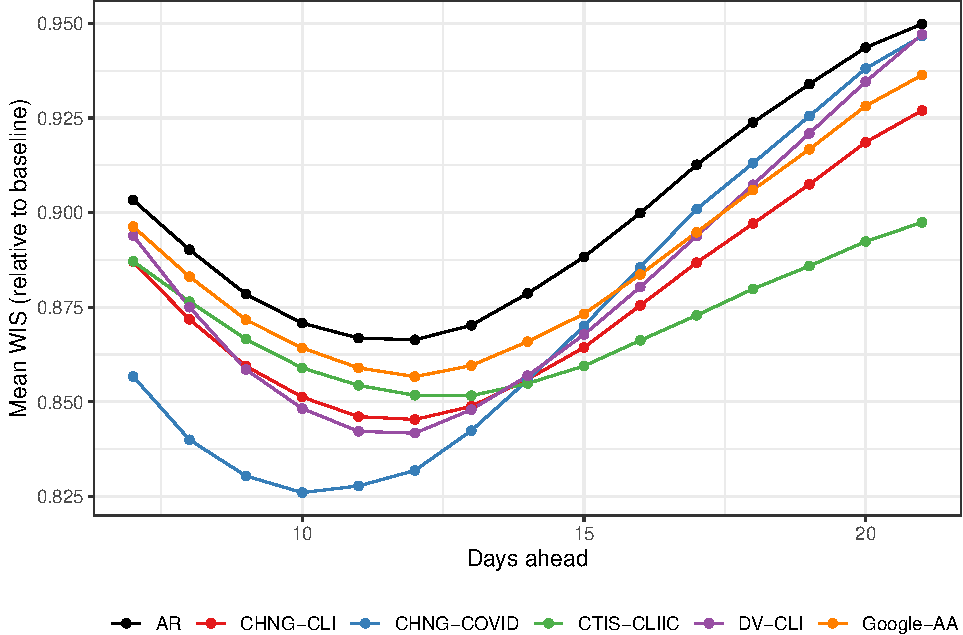
\includegraphics[width=\textwidth]{fig/fcast-finalized-1} 

}

\caption{Forecasting performance using finalized data. Compare to Figure 3 in the manuscript.}\label{fig:fcast-finalized}
\end{figure}

\clearpage

\begin{figure}

{\centering 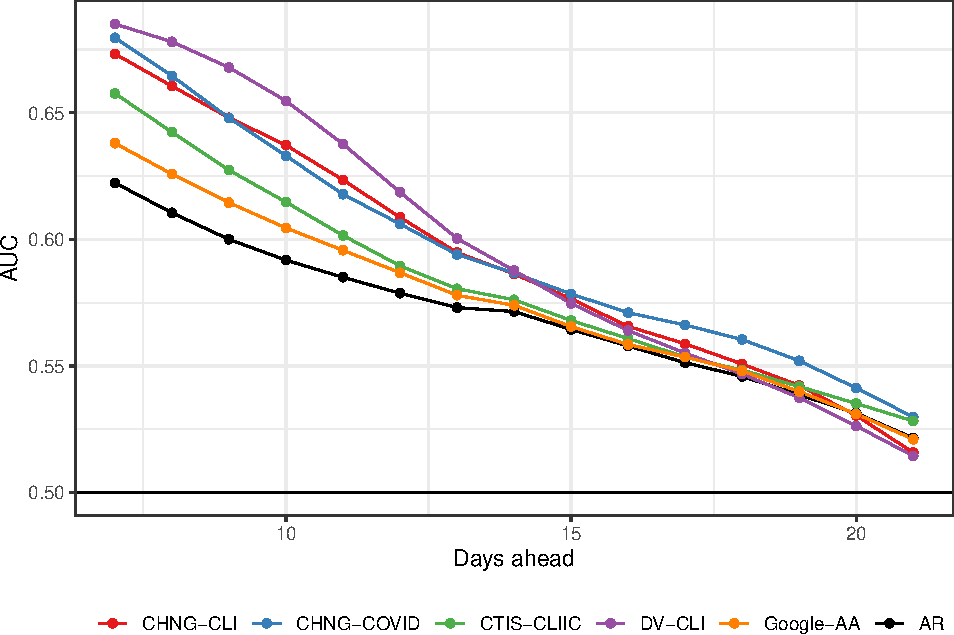
\includegraphics[width=\textwidth]{fig/hot-finalized-1} 

}

\caption{Hotspot prediction performance using finalized data. Compare to Figure 4 in the manuscript.}\label{fig:hot-finalized}
\end{figure}

\clearpage

\begin{figure}

{\centering 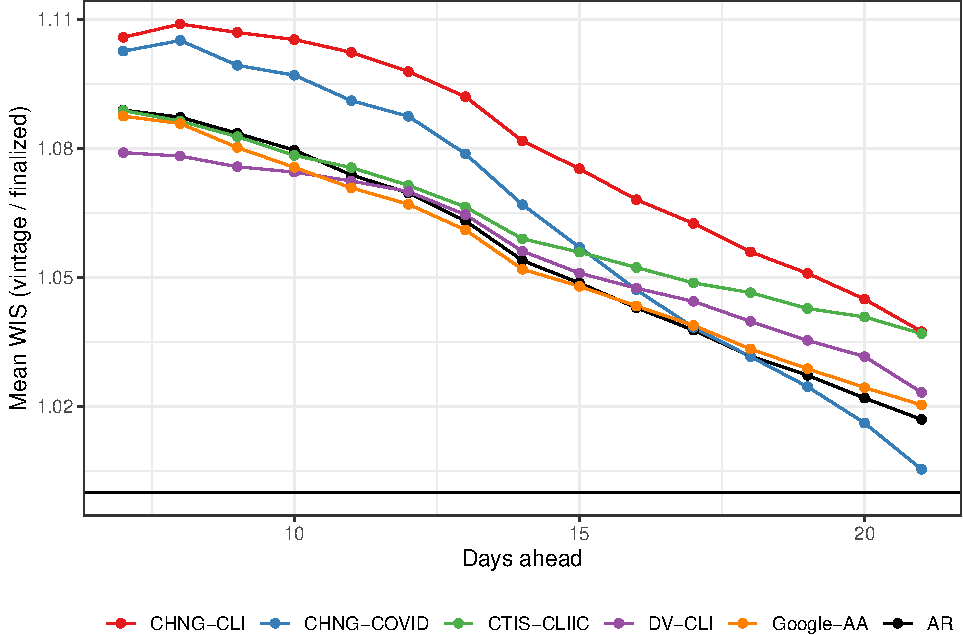
\includegraphics[width=\textwidth]{fig/fcast-honest-v-finalized-1} 

}

\caption{Relative forecast WIS with vintage compared to finalized data. Using finalized data leads to overly optimistic performance.}\label{fig:fcast-honest-v-finalized}
\end{figure}

\clearpage

\begin{figure}

{\centering 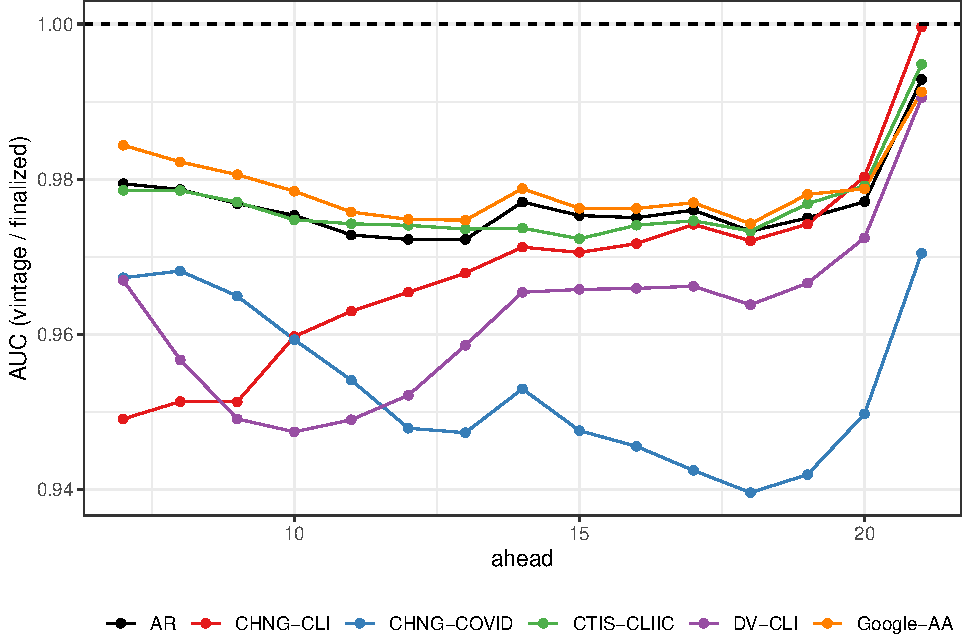
\includegraphics[width=\textwidth]{fig/hot-honest-v-finalized-1} 

}

\caption{Relative AUC with vintage compared to finalized data. Using finalized data leads to overly optimistic hotspot performance.}\label{fig:hot-honest-v-finalized}
\end{figure}

\clearpage

\begin{figure}

{\centering 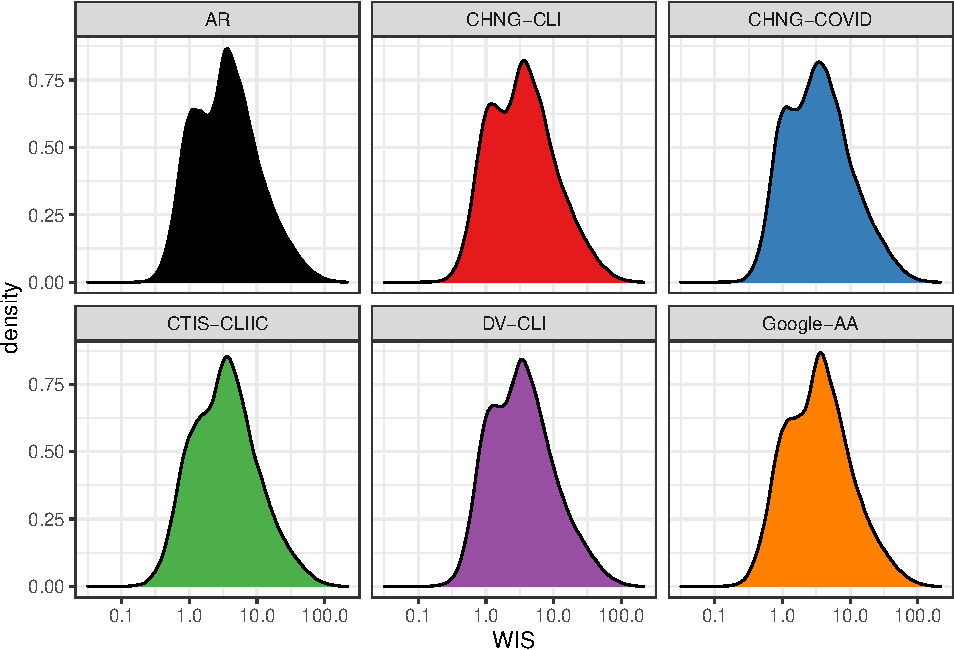
\includegraphics[width=\textwidth]{fig/wis-densities-1} 

}

\caption{Weighted interval score appears to more closely resemble a log-Gaussian distribution.}\label{fig:wis-densities}
\end{figure}

\clearpage

\begin{figure}

{\centering 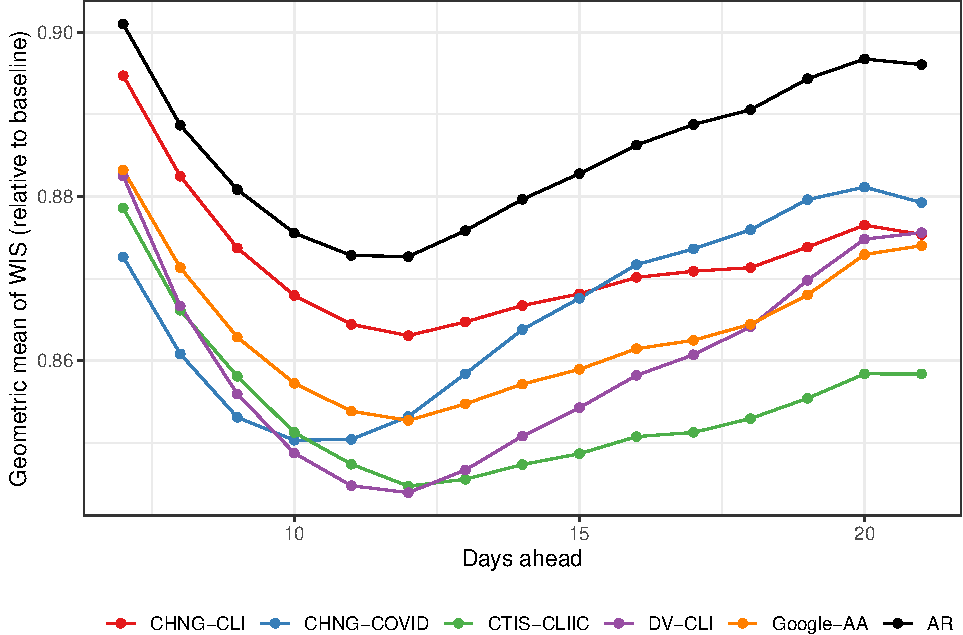
\includegraphics[width=\textwidth]{fig/fcast-adjusted-1} 

}

\caption{Relative forecast performance using vintage data and summarizing with the more robust geometric mean.}\label{fig:fcast-adjusted}
\end{figure}

\clearpage

\begin{figure}

{\centering 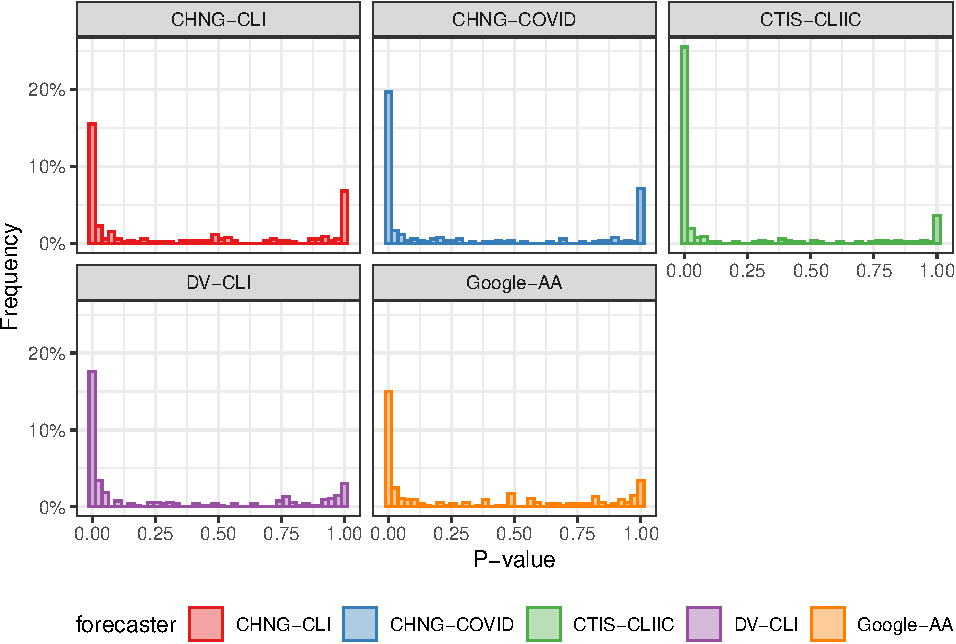
\includegraphics[width=\textwidth]{fig/sign-test-1} 

}

\caption{P-values for a sign test that the WIS of the AR forecaster is smaller than that of the indicator-assisted model. Each P-value corresponds a particular forecast date.}\label{fig:sign-test}
\end{figure}

\begin{table}

\caption{\label{tab:dm-test}$P$-values for a Diebold-Mariano test for differences in forecast error. The test is for the null hypothesis of equal performance against the alternative that the indicator assisted model is better.}
\centering
\begin{tabular}[t]{lrrrrr}
\toprule
metric & CHNG-CLI & CHNG-COVID & CTIS-CLIIC & DV-CLI & Google-AA\\
\midrule
Geometric Mean Relative WIS & 0.141 & 0.076 & 0.000 & 0.059 & 0.008\\
Mean Relative WIS & 0.186 & 0.137 & 0.002 & 0.074 & 0.064\\
\bottomrule
\end{tabular}
\end{table}

\begin{figure}

{\centering 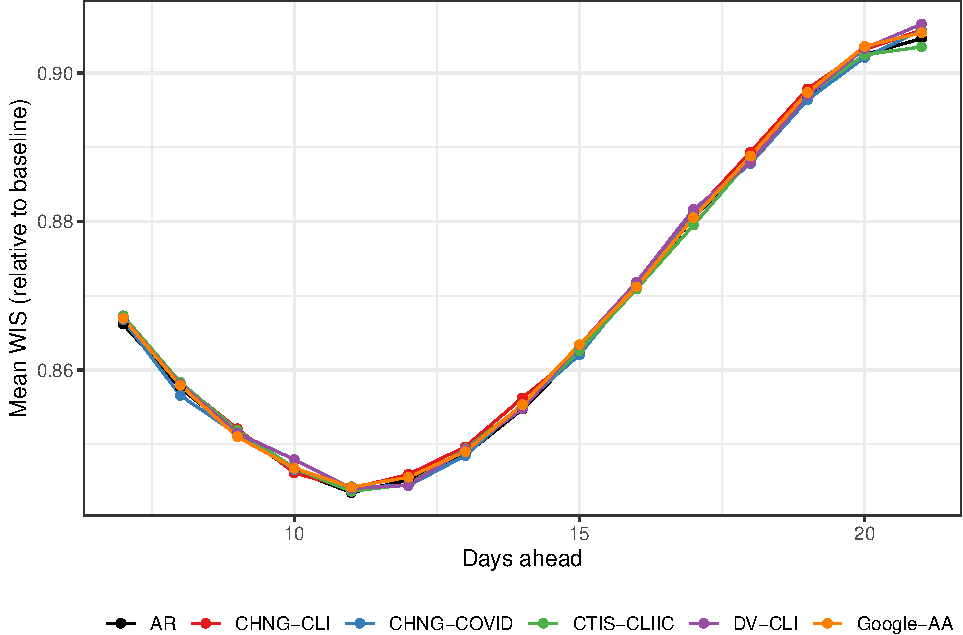
\includegraphics[width=\textwidth]{fig/fcast-booted-1} 

}

\caption{Forecast performance when indicators are replaced with samples from their empirical distribution. Performance is largely similar to the AR model.}\label{fig:fcast-booted}
\end{figure}

\clearpage

\begin{figure}

{\centering 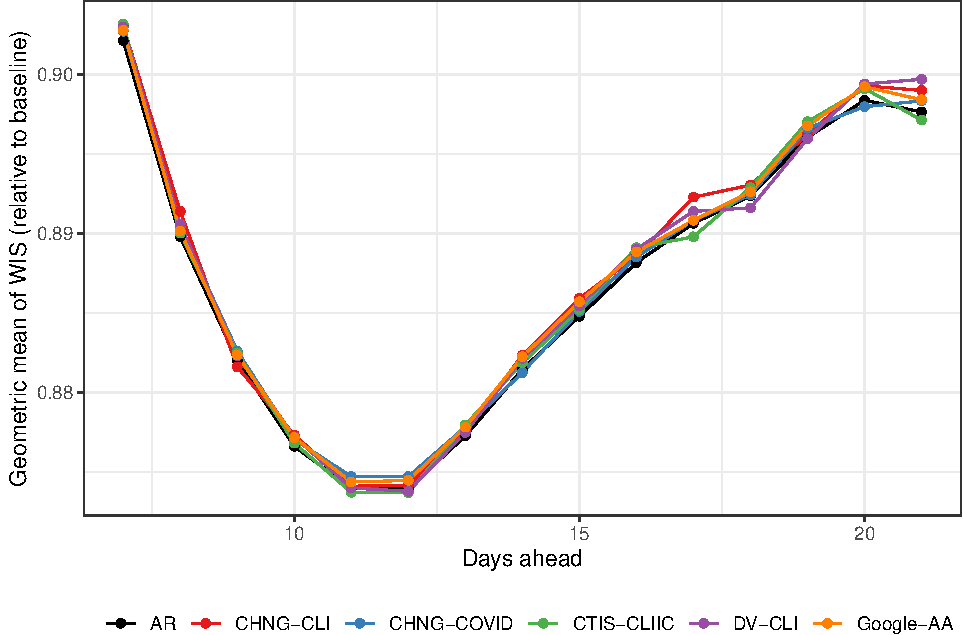
\includegraphics[width=\textwidth]{fig/fcast-booted-adjusted-1} 

}

\caption{Forecast performance as measured with the geometric mean when indicators are replaced with samples from their empirical distribution. Performance is largely similar to the AR model.}\label{fig:fcast-booted-adjusted}
\end{figure}

\clearpage

\begin{figure}

{\centering 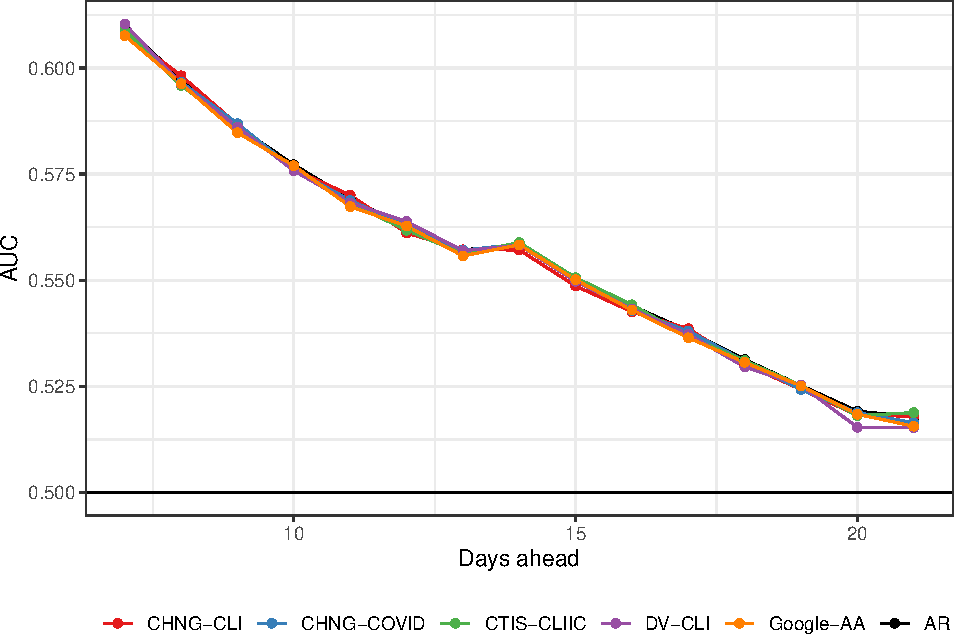
\includegraphics[width=\textwidth]{fig/hot-booted-1} 

}

\caption{Hotspot prediction performance when indicators are replaced with samples from their empirical distribution. Performance is largely similar to the AR model.}\label{fig:hot-booted}
\end{figure}

\clearpage

\begin{figure}

{\centering 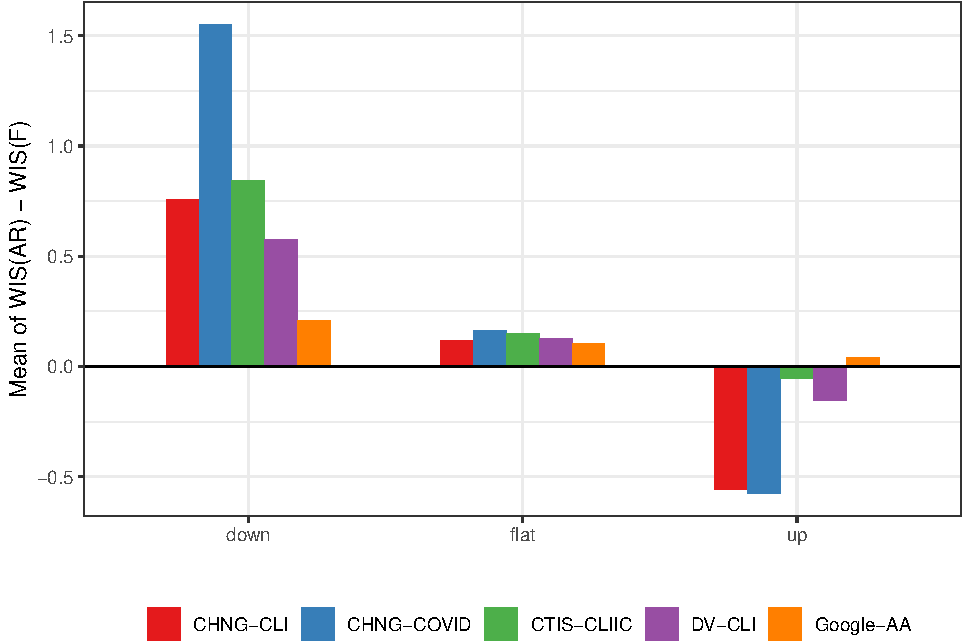
\includegraphics[width=\textwidth]{fig/upswing-summary-1} 

}

\caption{Average difference between the WIS of the AR model and the WIS of the other forecasters. The indicator-assisted forecasters do best during down and flat periods.}\label{fig:upswing-summary}
\end{figure}

\clearpage

\begin{figure}

{\centering 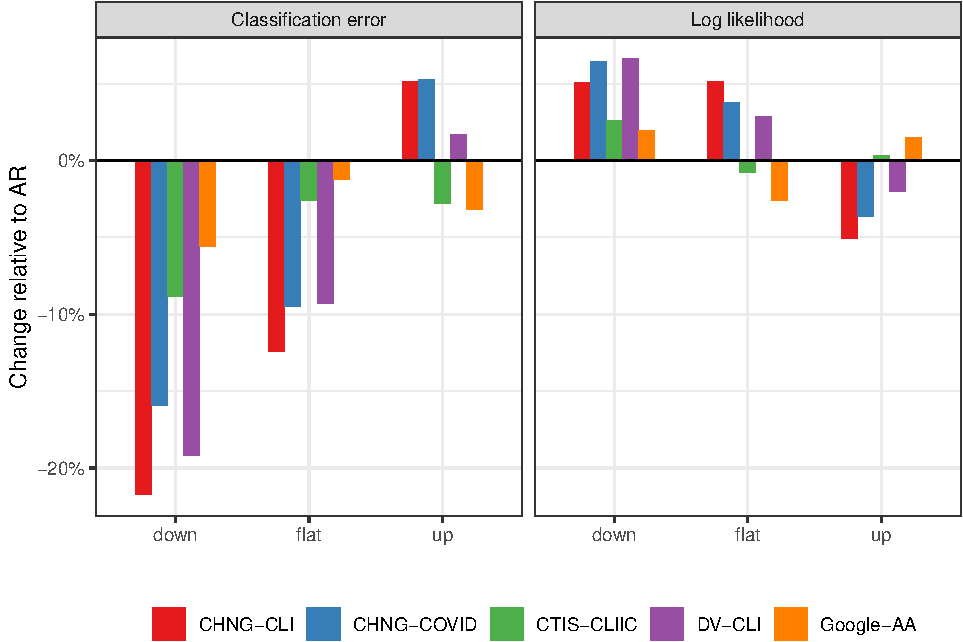
\includegraphics[width=\textwidth]{fig/hotspots-upswing-downswing-1} 

}

\caption{Classification and loglikelihood separated into periods of upswing, downswing, and flat cases. Like the analysis of the forecasting task in the main paper (see Figure 7), performance is better during down and flat periods.}\label{fig:hotspots-upswing-downswing}
\end{figure}

\clearpage

\begin{figure}

{\centering 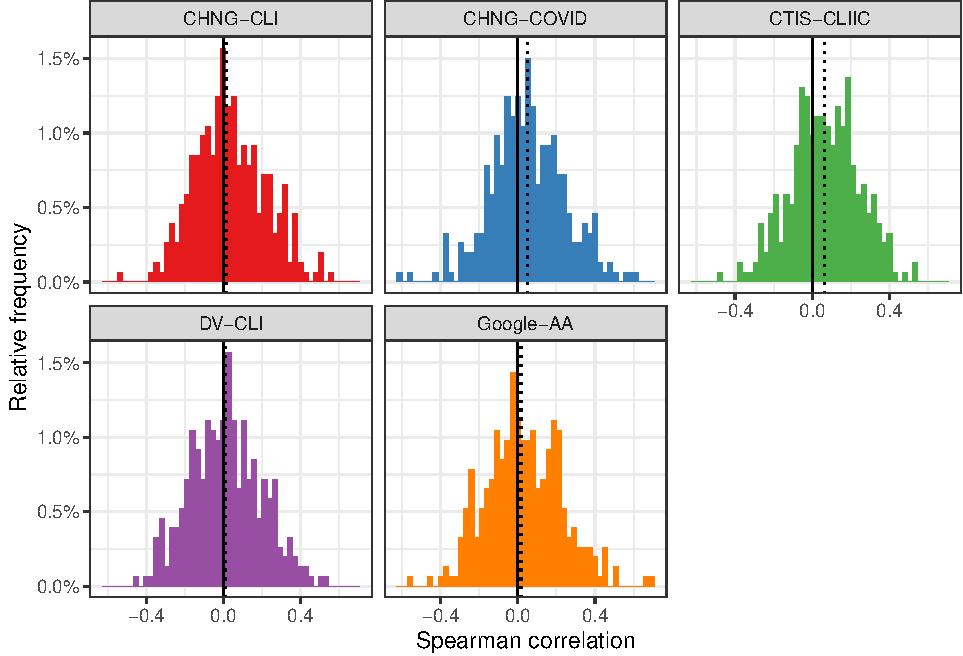
\includegraphics[width=\textwidth]{fig/cor-wis-ratio-1} 

}

\caption{Histograms of the Spearman correlation between the ratio of AR to AR WIS with the percent change in smoothed case rates relative to 7 days earlier.}\label{fig:cor-wis-ratio}
\end{figure}

\clearpage

\clearpage

\begin{figure}

{\centering 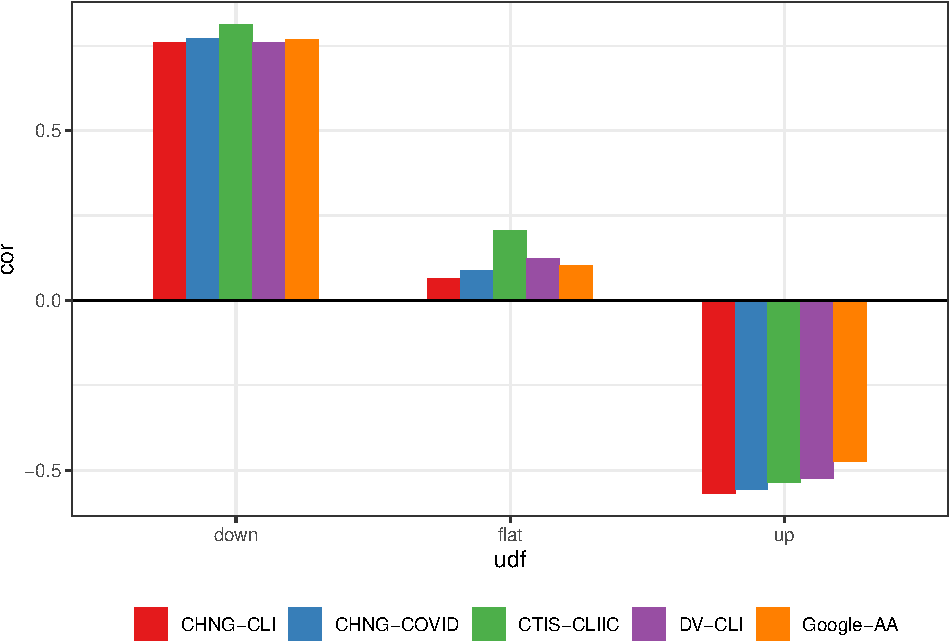
\includegraphics[width=\textwidth]{fig/upswing-corr-table-1} 

}

\caption{Correlation of the difference in WIS with the difference in median predictions for the AR model relative to the indicator-assisted forecaster. In down periods, improvements in forecast risk are highlycorrelated with lower median predictions. The opposite is true in up periods. This suggests, as one might expect that improved performance of the indicator-assisted model is attributable to being closer to the truth then the AR model. This conclusion is stronger in down periods then in up periods.}\label{fig:upswing-corr-table}
\end{figure}

\clearpage

\begin{figure}

{\centering 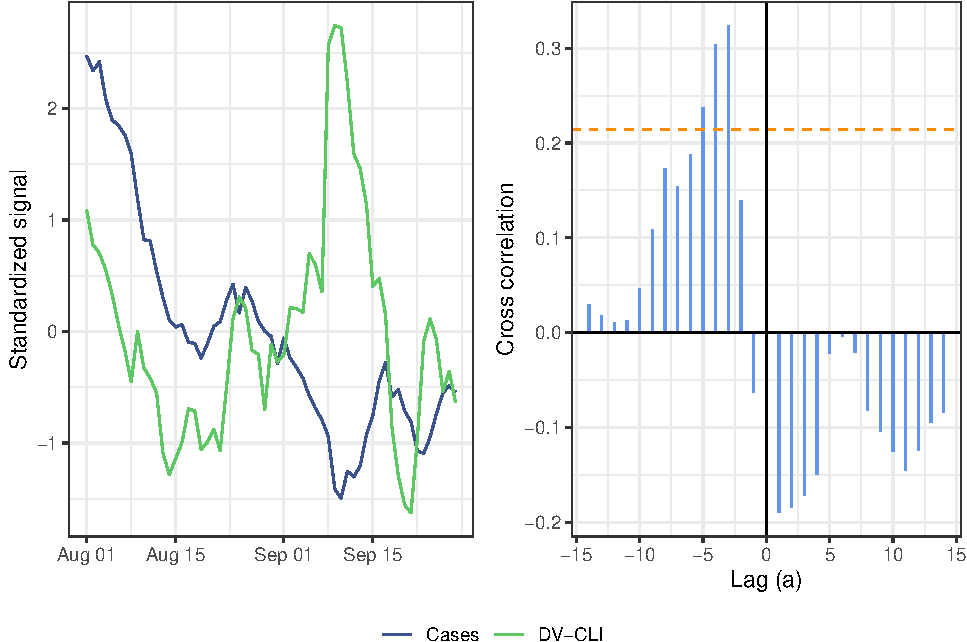
\includegraphics[width=\textwidth]{fig/ccf-dv-finalized-1} 

}

\caption{Illustration of the cross-correlation function between DV-CLI and cases. The left panel shows the standardized signals over the period from August 1 to September 28 (as of May 15, 2021). The right panel shows $\CCF_{\ell}(a)$ for different values of $a$ as vertical blue bars. The orange dashed lines indicate the 95\% significance threshold. By our leadingness/laggingness metric, DV-CLI is leading (but notlagging) cases over this period.}\label{fig:ccf-dv-finalized}
\end{figure}

\clearpage

\begin{figure}

{\centering 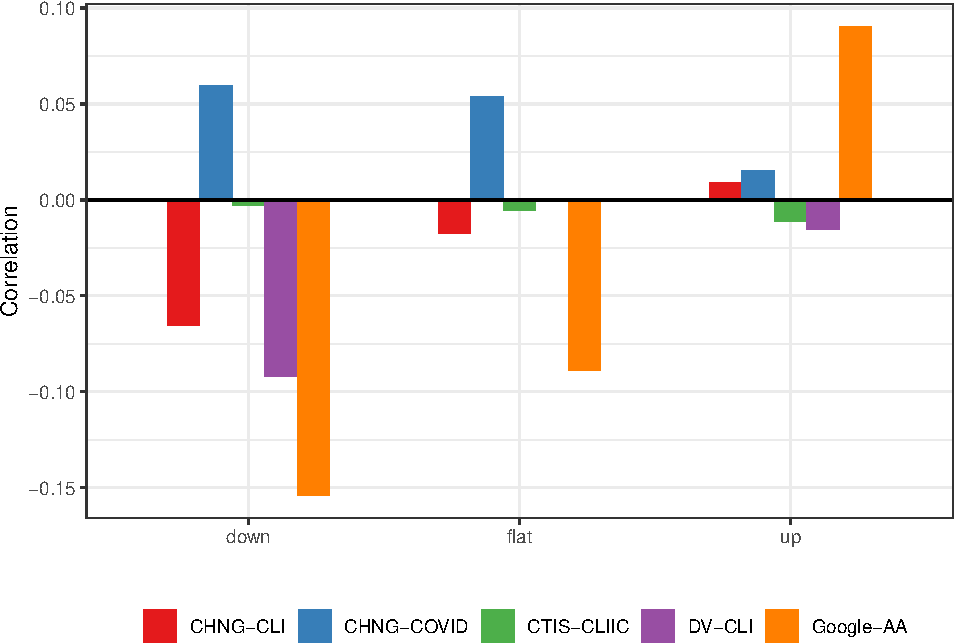
\includegraphics[width=\textwidth]{fig/lagging-only-1} 

}

\caption{Correlation of the difference in WIS with the  laggingness of the indicator at the target date, stratified by up, down, or flat period. Compare to Figure 5 in the manuscript.}\label{fig:lagging-only}
\end{figure}

\clearpage

\begin{figure}

{\centering 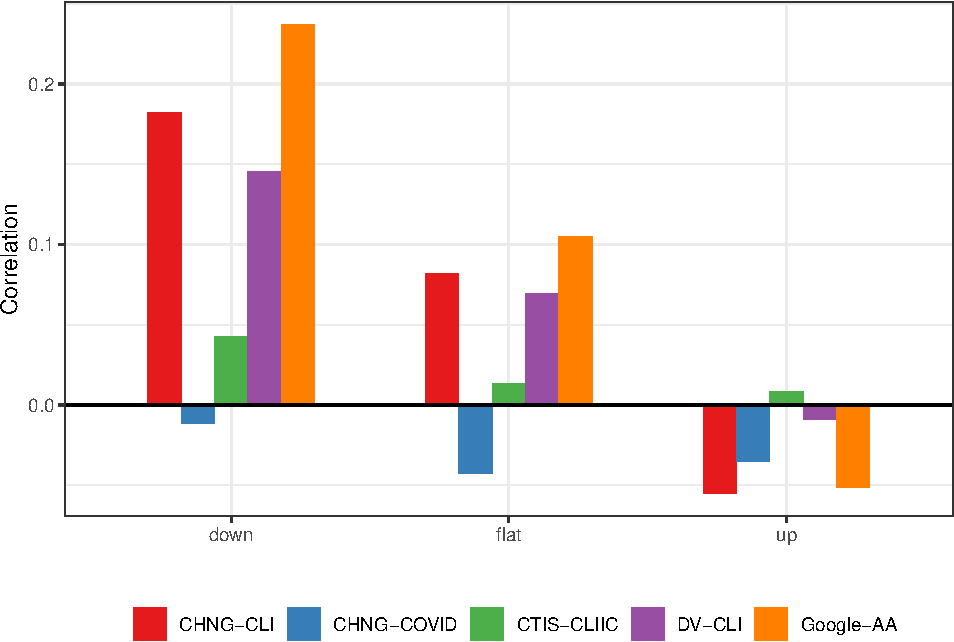
\includegraphics[width=\textwidth]{fig/diff-in-lead-lag-1} 

}

\caption{Correlation of the difference between leadingness and laggingness with the difference in WIS. The relationship is essentially the same as described in the manuscript and shown in Figure 5.}\label{fig:diff-in-lead-lag}
\end{figure}

\clearpage

\begin{figure}

{\centering 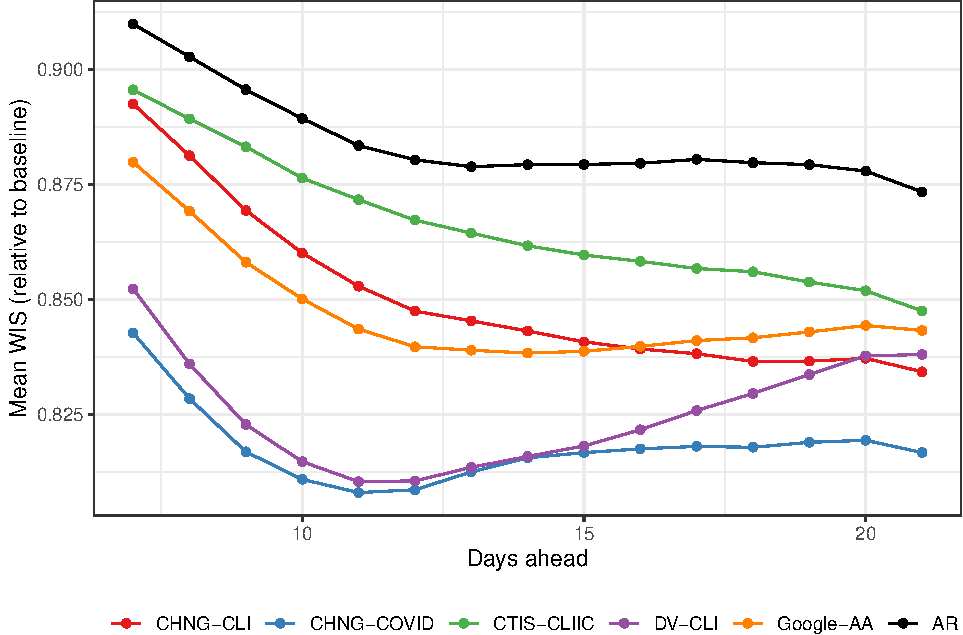
\includegraphics[width=\textwidth]{fig/fcast-alldates-1} 

}

\caption{Forecast performance over all periods. Performance largely improves for all forecasters with the inclusion of data in 2021.}\label{fig:fcast-alldates}
\end{figure}

\clearpage

\begin{figure}

{\centering 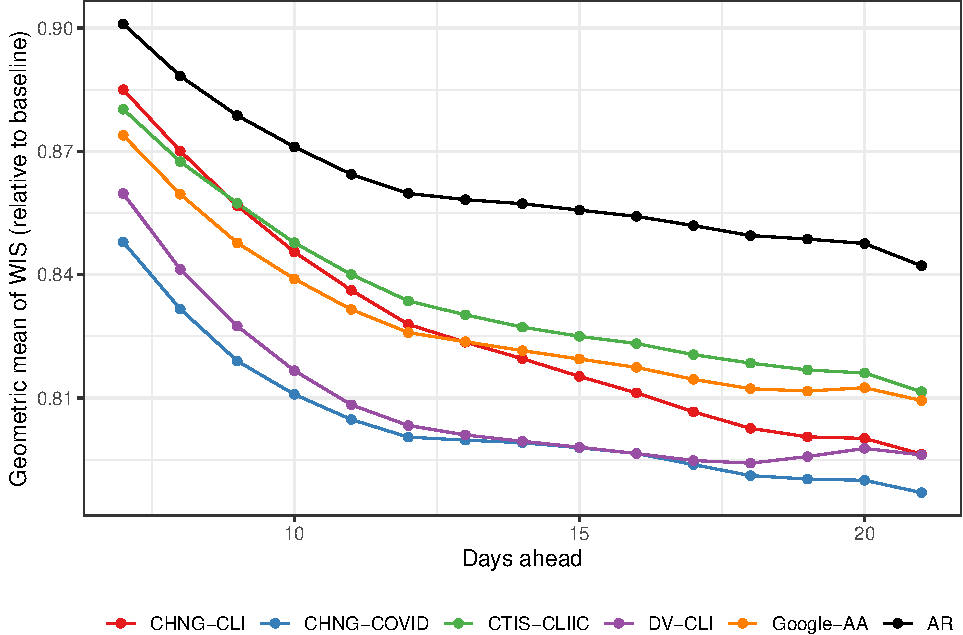
\includegraphics[width=\textwidth]{fig/fcast-alldates-adjusted-1} 

}

\caption{Forcast performance over all periods aggregaged with the geometric mean. Again, the inclusion of data in 2021 leads to improved performance.}\label{fig:fcast-alldates-adjusted}
\end{figure}

\clearpage

\begin{figure}

{\centering 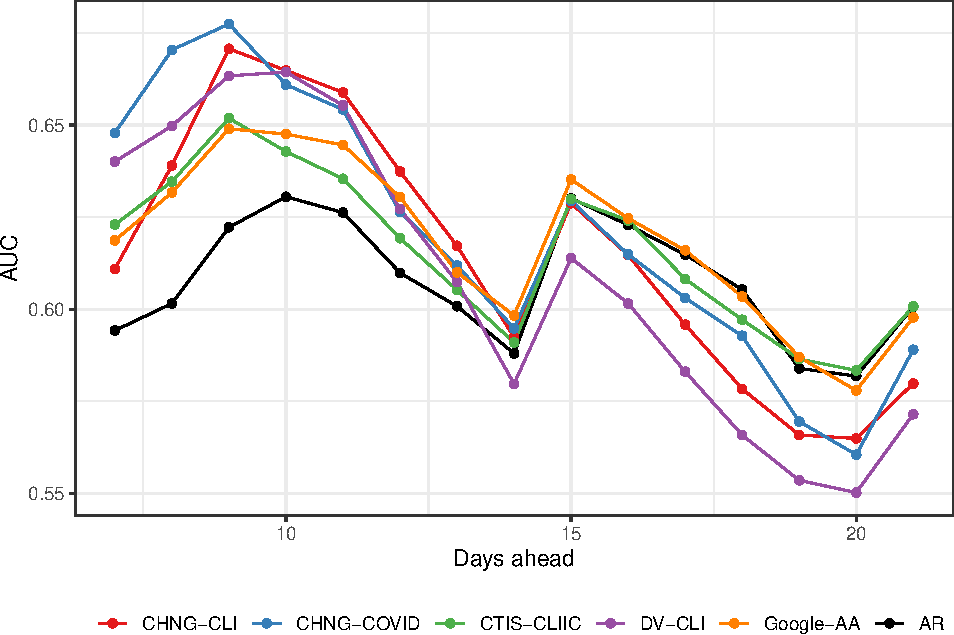
\includegraphics[width=\textwidth]{fig/hot-alldates-1} 

}

\caption{Area under the curve for hotspot predictions including data in 2021. Performance degrades relative to the period in 2020. However, there are far fewer hotspots during this period as case rates declined in much of the country.}\label{fig:hot-alldates}
\end{figure}

\clearpage


\FloatBarrier



\dataset{predictions.zip}{Archived {\tt .RDS} (R objects) files containing
  all predictions for forecasting and hotspots using vintage and finalized data.
Persistent DOI to be added at publication.}

\dataset{evaluations.zip}{Archived {\tt .RDS} (R objects) files containing
  all evaluations for forecasting and hotspots using vintage and finalized data.
  Persistent DOI to be added at publication.}

\dataset{analysis.zip}{Archived {\tt .RDS} (R objects) files containing
  additional data used to produce graphics and conclusions in the manuscript.
  Persistent DOI to be added at publication.}

\dataset{code.zip}{R script files containing
  all code used to reproduce the analysis described in the manuscript.
  Persistent DOI to be added at publication.}



\bibliography{../../common/covidcast.bib}

\end{document}